\chapter{Wybrane deskryptory cech}
\label{cha:deskryptory}

\section{HOG - Histogram of Oriented Gradients}
\label{sec:hog}

\subsection{Algorytm obliczenia deskryptora}

Algorytm obliczenia deskryptora cech HOG ma następującą postać:

\begin{algorithm}[H]
 \SetAlgoLined
 \KwData{obraz $n x m$ w przestrzeni barw RGB;\\$k$ - rozmiar komórki;\\$w$ - szerokość histogramu (tutaj 9)}
 \KwResult{wektor deskryptora cech o długości $\lfloor\frac{m}{k}\rfloor x \lfloor\frac{n}{k}\rfloor x w$}
 zamień przestrzeń barw RGB na skalę szarości\;
 oblicz gradient w obu kierunkach na obrazie np. używając maski  $\left[\begin{array}{ccc}1 & 0 & -1\end{array}\right]$\;
 dla każdego piksela obrazu oblicz długość wektora gradientu ($\sqrt{I_x^2 + I_y^2}$) oraz jego kąt, tak aby leżał w przedziale $[0; \pi]$ (wykorzystując funkcję $atan2(I_y, I_x)$)\;
 podziel obraz na komórki $k x k$\;
 dla każdej komórki utwórz histogram o szerokości $w$, gdzie cechą jest kąt z przedziału $[0; \pi]$, a liczebnością suma długości gradientów\;
 \ForEach{piksel $\in$ obraz}{
	dokonaj interpolacji dwuliniowej współrzędnych piksela względem środków czterech najbliższych komórek\;
	w histogramach odpowiadającym powyższym komórkom zwiększ liczebność kątom, po przeprowadzaniu interpolacji liniowej kąta odpowiadającemu pikselowi\;
 }
 dokonaj normalizacji każdej próbki (w niniejszej pracy jest to norma L2)\;
 połącz kolejne wiersze macierzy próbek w wektor\;
 \Return{wektor cech}\;
 \caption{Algorytm obliczenia deskryptora cech HOG}
\end{algorithm}

\subsection{Wyniki pierwszej walidacji}

W tabeli \ref{tab:hog_first} zestawiono wyniki krzyżowej walidacji pierwszego klasyfikatora wytrenowanego 
próbkami, uzyskanymi metodą HOG, w zależności od rozmiaru komórki, w której wyliczany był histogram orientacji gradientów.

\begin{center}
    \begin{longtable}{ | p{5cm} | p{3cm} | p{3cm} | p{3cm} |}
    \caption{Wyniki pierwszej walidacji krzyżowej przy użyciu deskryptora HOG}
    \label{tab:hog_first} \\
    \hline
	Rozmiar komórki & 8x8 & 12x12 & 16x16 \\ \hline
	Funkcja jądra SVM & liniowa & liniowa & liniowa  \\ \hline
    Długość wektora cech & 7308 & 800 & 512 \\ \hline
    Liczba pozytywnych detekcji w pozytywnym zbiorze testowym & 575 & 474 & 462 \\ \hline
    Liczba negatywnych detekcji w pozytywnym zbiorze testowym & 57 & 152 & 164 \\ \hline
    Celność metody w pozytywnym zbiorze testowym & \textbf{91,85\%} & \textbf{75,72\%} & \textbf{73,81\%} \\ \hline
    Liczba pozytywnych detekcji w negatywnych zbiorze testowym & 31 & 172 & 57 \\ \hline
    Liczba negatywnych detekcji w negatywnym zbiorze testowym & 875 & 734 & 849 \\ \hline
    Celność metody w negatywnym zbiorze testowym & \textbf{96,58\%} & \textbf{81,02\%} & \textbf{93,71\%} \\ \hline
    \end{longtable}
\end{center}

\subsection{Przykłady fałszywych detekcji}

Przeważającą część fałszywie pozytywnych detekcji uzyskiwanych metodą HOG są okna, w których występują pary długich, równoległych linii, przypominające ludzką sylwetkę czy elementy które kształtem przypominają ludzką twarz. Jest to spodziewany efekt, biorąc pod uwagę to jak budowany jest deskryptor cech (opisywany jest kształt na podstawie krawędzi obrazu wejściowego).
Liczby wygenerowanych fałszywie pozytywnych okien, w zależności od rozmiaru komórki, przedstawione zostały w tabeli \ref{tab:fp_hog}.
Przykładowe fałszywie pozytywne detekcje dla metody HOG zostały przedstawione na rysunku \ref{fig:fp_hog}.

\begin{figure}[htb]
\centering
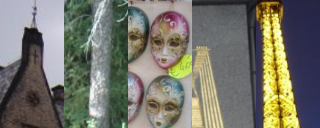
\includegraphics[width=0.8\textwidth]{hog_fps.png}
\caption{Przykłady fałszywie pozytywnych detekcji w metodzie HOG}
\label{fig:fp_hog}
\end{figure}

\begin{center}
    \begin{longtable}{ | p{5cm} | p{3cm} | p{3cm} | p{3cm} |}
    \caption{Liczba znalezionych fałszywie pozytywnych okien przy użyciu deskryptora HOG} \\
    \hline
	Rozmiar komórki & 8x8 & 12x12 & 16x16 \\ \hline
	Funkcja jądra SVM & liniowa & liniowa & liniowa  \\ \hline
    Liczba znalezionych pozytywnie fałszywych okien & 2759 & 14538 & 6446 \\ \hline
    \end{longtable}
    \label{tab:fp_hog}
\end{center}

\subsection{Wyniki drugiej walidacji}

W tabeli \ref{tab:hog_second} zestawiono wyniki krzyżowej walidacji klasyfikatora po dotrenowaniu pierwszego klasyfikatora fałszywie pozytywnymi detekcjami, wykrytymi w zbiorze testowym. W celu zminimalizowania efektu przetrenowania klasyfikatora wzięto pod uwagę tylko 25\% wygenerowanego zbioru.

\begin{center}
    \begin{longtable}{ | p{5cm} | p{3cm} | p{3cm} | p{3cm} |}
    \caption{Wyniki drugiej walidacji krzyżowej przy użyciu deskryptora HOG} 
    \label{tab:hog_second}\\
    \hline
	Rozmiar komórki & 8x8 & 12x12 & 16x16 \\ \hline
	Funkcja jądra SVM & liniowa & liniowa & liniowa  \\ \hline
    Liczba pozytywnych detekcji w pozytywnym zbiorze testowym & 531 & 445 & 223 \\ \hline
    Liczba negatywnych detekcji w pozytywnym zbiorze testowym & 95 & 181 & 403 \\ \hline
    Celność metody w pozytywnym zbiorze testowym & \textbf{84,82\%} & \textbf{71,09\%} & \textbf{35,62\%} \\ \hline
    Liczba pozytywnych detekcji w negatywnych zbiorze testowym & 32 & 79 & 290 \\ \hline
    Liczba negatywnych detekcji w negatywnym zbiorze testowym & 874 & 827 & 614 \\ \hline
    Celność metody w negatywnym zbiorze testowym & \textbf{96,47\%} & \textbf{91,28\%} & \textbf{67,77\%} \\ \hline
    \end{longtable}
\end{center}

\clearpage

\subsection{Rozkłady błędów detekcji}

Wykres rozkładu błędu detekcji dla metody HOG zaprezentowany został na rysunku \ref{fig:hog_det}.
Na osi odciętych wykresu znajduje się rząd stosunku fałszywych pozytywnych detekcji klasyfikatora i wszystkich negatywnych testowanych okien, na osi rzędnych zaś, średni odsetek błędu klasyfikatora w detekcji pozytywnego okna. Na podstawie wykresu można wyciągnąć wniosek, że w przypadku użycia liniowej funkcji jądra klasyfikatora SVM, najlepsze zachowanie prezentuje klasyfikator zbudowany przy deskryptora HOG wyliczanego na komórkach o rozmiarze 8x8 pikseli. Zachowuje on bardzo dobry wynik detekcji obiektu (ok. 95\%), w przypadku, gdy liczba FPPW jest rzędu $10^{-2}$. Na podstawie wykresu można również stwierdzić, że przy wyliczaniu bloków o rozmiarze 16x16 pikseli deskryptor HOG jest złym deskryptorem, a stopień jego błędu detekcji rośnie aż do 70\% przy FPPW rzędu $10^{-3}$.

\begin{figure}[htb]
\centering
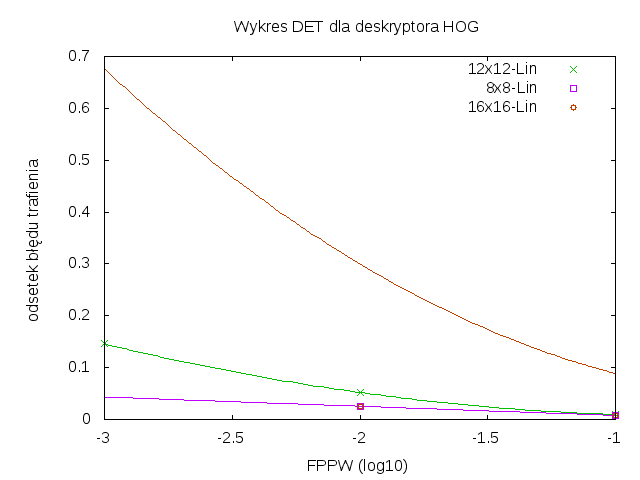
\includegraphics[width=0.9\textwidth]{hog_det.png}
\caption{Rozkład błędu detekcji dla różnych przyjętych komórek}
\label{fig:hog_det}
\end{figure}

\subsection{Analiza złożoności poszczególnych kroków metody}

W tabeli \ref{tab:hog_times} zestawiono czasy wykonywania poszczególnych kroków metodologii, w zależności od rozmiaru komórki deskryptora HOG, na konfiguracji testowej.

\begin{center}
    \begin{longtable}{ | p{5cm} | p{3cm} | p{3cm} | p{3cm} |}
    \caption{Czas wykonywania poszczególnych etapów badania metody HOG}
    \label{tab:hog_times}\\
    \hline
	Rozmiar komórki & 8x8 & 12x12 & 16x16 \\ \hline
	Funkcja jądra SVM & liniowa & liniowa & liniowa  \\ \hline
    Ekstrakcja cech pozytywnych / próbka & 6,23 ms & 5,67 ms & 5,19 ms \\ \hline
    Ekstrakcja cech negatywnych / próbka & 5,27 ms & 4,80 ms & 4,28 ms \\ \hline
    Pierwszy trening klasyfikatora & 33,69 s & 12,67 s & 8,14 s \\ \hline
    Generacja fałszywie pozytywnych okien & 590,40 s & 455,72 s & 409,20 s \\ \hline
    Drugi trening klasyfikatora & 40,62 s & 18,88 s & 10,36 s \\ \hline
    Analiza rozkładu błędu detekcji w zbiorze testowym & 1938 s & 1353 s & 1228 s \\ \hline
    \end{longtable}
\end{center}

\subsection{Podsumowanie}

Na podstawie uzyskanych wyników można stwierdzić, że najskuteczniejszą z przetestowanych wielkości komórki w deskryptorze HOG jest ta o rozmiarze 8x8 pikseli. Jako jedyna daje ona rozsądne wyniki przy obydwu walidacjach klasyfikatora. Również rozkład DET dla takiej wielkości komórki sugeruje wysoką skuteczność działania.

\clearpage

\section{Macierz kowariancji cech}
\label{sec:cov}

\subsection{Algorytm obliczenia deskryptora}

Algorytm obliczenia deskryptora cech, wykorzystującego macierz kowariancji ma następującą postać:

\begin{algorithm}[H]
 \SetAlgoLined
 \KwData{obraz $n x m$ w przestrzeni barw RGB;\\$k$ - rozmiar lokalnego bloku}
 \KwResult{wektor deskryptora cech o długości $\lfloor\frac{m}{k}\rfloor x \lfloor\frac{n}{k}\rfloor x 6^{2}$}
 macierz próbek := $\left[\begin{array}{ccc}\end{array}\right]$\;
 zamień przestrzeń barw RGB na skalę szarości\;
 podziel obraz na bloki $k x k$\;
 \ForEach{blok}{
	$I_x$ := jednokrotny operator Sobela dla bloku w kierunku poziomym\;
	$I_y$ := jednokrotny operator Sobela dla bloku w kierunku pionowym\;
	$I_{xx}$ := dwukrotny operator Sobela dla bloku w kierunku poziomym\;
	$I_{yy}$ := dwukrotny operator Sobela dla bloku w kierunku pionowym\;
	macierz cech := $\left[\begin{array}{ccc}\end{array}\right]$\;
	\ForEach{piksel $\in$ okno} {
		wektor cech := $\left[\begin{array}{cccccc}\vert I_x \vert & \vert I_y \vert & \vert I_{xx} \vert & \vert I_{yy} \vert & \sqrt{I_x^2 + I_y^2} & atan2(I_y, I_x)\end{array}\right]$\;
		dodaj wektor cech jako wiersz do macierzy cech\;
	}
	oblicz macierz kowariancji macierzy cech\;
	połącz kolejne wiersze macierzy cech w jeden wektor\;
	dodaj wektor do macierzy próbek\;
 }
 dokonaj normalizacji każdej próbki (w niniejszej pracy jest to norma L2)\;
 połącz kolejne wiersze macierzy próbek w wektor\;
 \Return{wektor cech}\;
 \caption{Algorytm obliczenia deskryptora cech, wykorzystującego macierz kowariancji}
\end{algorithm}

\subsection{Wyniki pierwszej walidacji}

W tabeli zestawiono wyniki krzyżowej walidacji pierwszego klasyfikatora wytrenowanego 
próbkami, uzyskanymi na podstawie wyliczenia deskryptora cech, wykorzystującego macierz kowariancji, w zależności od rozmiaru bloku na obrazie, w którym liczono macierz kowariancji.

\begin{center}
    \begin{longtable}{ | p{5cm} | p{3cm} | p{3cm} | p{3cm} |}
    \caption{Wyniki pierwszej walidacji krzyżowej przy użyciu deskryptora wykorzystującego macierz kowariancji cech}
    \label{tab:cov_first}\\
    \hline
	Rozmiar bloku & 8x8 & 16x16 & 24x24 \\ \hline
	Funkcja jądra SVM & liniowa & liniowa & liniowa  \\ \hline
    Długość wektora cech & 4608 & 832 & 360 \\ \hline
    Liczba pozytywnych detekcji w pozytywnym zbiorze testowym & 599 & 593 & 584 \\ \hline
    Liczba negatywnych detekcji w pozytywnym zbiorze testowym & 27 & 33 & 42 \\ \hline
    Celność metody w pozytywnym zbiorze testowym & \textbf{95,69\%} & \textbf{94,73\%} & \textbf{93,29\%} \\ \hline
    Liczba pozytywnych detekcji w negatywnych zbiorze testowym & 21 & 30 & 29 \\ \hline
    Liczba negatywnych detekcji w negatywnym zbiorze testowym & 885 & 876 & 877 \\ \hline
    Celność metody w negatywnym zbiorze testowym & \textbf{97,68\%} & \textbf{96,69\%} & \textbf{96,80\%} \\ \hline
    \end{longtable}
\end{center}

\subsection{Przykłady fałszywych detekcji}

Podobnie jak w przypadku metody HOG, zdecydowaną część zbioru fałszywie pozytywnych detekcji stanowiły okna, w których znajdowały się obiekty mające kształty przypominające ludzkie sylwetki, czyli np. obiekty zajmujące większość część okna, posiadające parę długich, równoległych krawędzi, jak słup czy drzewo.
Liczby wygenerowanych fałszywie pozytywnych okien, w zależności od rozmiaru komórki, przedstawione zostały w tabeli \ref{tab:fp_cov}.
Przykładowe fałszywie pozytywne detekcje dla metody opierającej się na liczeniu macierzy kowariancji cech, zostały przedstawione na rysunku \ref{fig:fp_cov}.

\begin{figure}[htb]
\centering
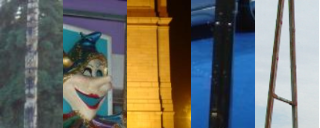
\includegraphics[width=0.8\textwidth]{cov_fps.png}
\caption{Przykłady fałszywie pozytywnych detekcji w metodzie korzystającej z macierzy kowariancji cech}
\label{fig:fp_cov}
\end{figure}

\begin{center}
    \begin{longtable}{ | p{5cm} | p{3cm} | p{3cm} | p{3cm} |}
    \caption{Liczba znalezionych fałszywie pozytywnych okien przy użyciu macierzy kowariancji cech} \\
    \hline
	Rozmiar komórki & 8x8 & 16x16 & 24x24 \\ \hline
	Funkcja jądra SVM & liniowa & liniowa & liniowa  \\ \hline
    Liczba znalezionych pozytywnie fałszywych okien & 4271 & 4141 & 7513 \\ \hline
    \end{longtable}
    \label{tab:fp_cov}
\end{center}

\subsection{Wyniki drugiej walidacji}

W \ref{tab:cov_second} tabeli zestawiono wyniki krzyżowej walidacji klasyfikatora po dotrenowaniu pierwszego klasyfikatora fałszywymi pozytywnymi detekcjami, wykrytymi w zbiorze testowym. W celu zminimalizowania efektu przetrenowania klasyfikatora wzięto pod uwagę 25\% fałszywie pozytywnych detekcji wygenerowanych na zbiorze testowym.

\begin{center}
    \begin{longtable}{ | p{5cm} | p{3cm} | p{3cm} | p{3cm} |}
    \caption{Wyniki drugiej walidacji krzyżowej przy użyciu deskryptora wykorzystującego macierz kowariancji cech}
    \label{tab:cov_second} \\
    \hline
	Rozmiar bloku & 8x8 & 16x16 & 24x24 \\ \hline
	Funkcja jądra SVM & liniowa & liniowa & liniowa  \\ \hline
    Liczba pozytywnych detekcji w pozytywnym zbiorze testowym & 571 & 502 & 289 \\ \hline
    Liczba negatywnych detekcji w pozytywnym zbiorze testowym & 55 & 124 & 337 \\ \hline
    Celność metody w pozytywnym zbiorze testowym & \textbf{91,21\%} & \textbf{80,20\%} & \textbf{46,17\%} \\ \hline
    Liczba pozytywnych detekcji w negatywnych zbiorze testowym & 14 & 19 & 15 \\ \hline
    Liczba negatywnych detekcji w negatywnym zbiorze testowym & 892 & 887 & 891 \\ \hline
    Celność metody w negatywnym zbiorze testowym & \textbf{98,45\%} & \textbf{97,90\%} & \textbf{98,34\%} \\ \hline
    \end{longtable}
\end{center}


\subsection{Rozkłady błędów detekcji}

Wykres rozkładu błędu detekcji zaprezentowany został na rysunku \ref{fig:cov_det}. Na podstawie wykresu można wyciągnąć wniosek, że w przypadku użycia liniowej funkcji jądra klasyfikatora SVM, najlepsze zachowanie prezentuje klasyfikator zbudowany przy użyciu macierzy kowariancji wyliczanej na blokach 16x16. Zachowuje on rozsądny wynik detekcji obiektu, gdy ma on do czynienia z obrazem, gdzie liczba FPPW jest rzędu $10^{-2}$, a wraz z malejącą liczbą fałszywych pozytywnych detekcji, odsetek błędu detekcji nie rośnie zbyt gwałtownie, jak np. w przypadku deskryptora zbudowanego o macierz kowariancji wyliczaną na blokach 8x8.

\begin{figure}[htb]
\centering
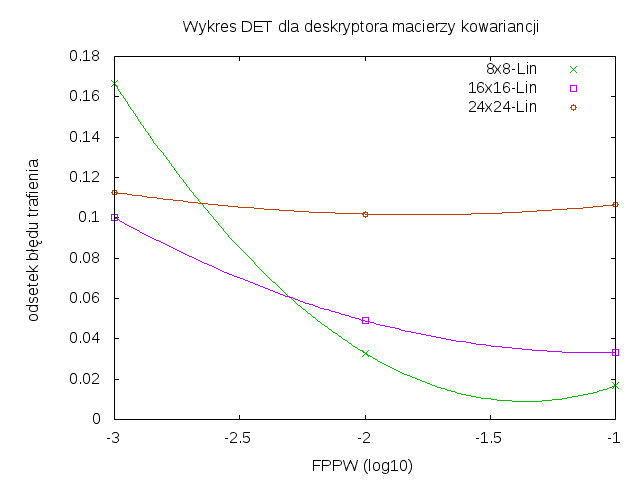
\includegraphics[width=0.9\textwidth]{cov_det.png}
\caption{Rozkład błędu detekcji dla różnych przyjętych wielkości macierzy}
\label{fig:cov_det}
\end{figure}

\subsection{Analiza złożoności poszczególnych kroków metody}

W tabeli \ref{tab:cov_times} zestawiono czasy wykonywania poszczególnych kroków metodologii, w zależności od rozmiaru bloku, z którego wyliczana jest macierz kowariancji, na konfiguracji testowej.

\begin{center}
    \begin{longtable}{ | p{5cm} | p{3cm} | p{3cm} | p{3cm} |}
    \caption{Czas wykonywania poszczególnych etapów badania metody opartej na macierzy kowariancji cech}
    \label{tab:cov_times}\\
    \hline
	Rozmiar bloku & 8x8 & 16x16 & 24x24 \\ \hline
	Funkcja jądra SVM & liniowa & liniowa & liniowa  \\ \hline
    Ekstrakcja cech pozytywnych / próbka & 11,12 ms & 4,33 ms & 3,51 ms \\ \hline
    Ekstrakcja cech negatywnych / próbka & 10,37 ms & 3,54 ms & 2,68 ms \\ \hline
    Pierwszy trening klasyfikatora & 50,81 s & 10,75 s & 5,99 s \\ \hline
    Generacja fałszywie pozytywnych okien & 909,12 s & 296,06 s & 231,88 s \\ \hline
    Drugi trening klasyfikatora & 68,49 s & 14,41 s & 8,79 s \\ \hline
    Analiza rozkładu błędu detekcji w zbiorze testowym & 3172 s & 912 s & 669 s \\ \hline
    \end{longtable}
\end{center}


\subsection{Podsumowanie}
Analizując powyższe wyniki można dojść do wniosku, że wielkościami bloków, dla których metoda daje rozsądne wyniki są bloki 8x8 pikseli i 16x16 pikseli. Użycie bloku 8x8 daje co prawda lepsze jakościowo wyniki w większości przypadków testowych, jednak jest to dużo bardziej kosztowne czasowo niż w przypadku bloku 16x16. Wynika to bezpośrednio z długości wektora cech, jaki powstaje w pierwszym przypadku. Deskryptor zbudowany na blokach o wielkości 24x24 pikseli jest złym deskryptorem i ma tendencję do szybkiego przetrenowania klasyfikatora.

\clearpage

\section{LBP - Local Binary Patterns}
\label{sec:lbp}

\subsection{Wprowadzenie}
W pracy \cite{Mu08} zaprezentowano metodę budowy deskryptora cech opartego na oryginalnym algorytmie Local Binary Patterns, dającego jednak lepsze wyniki w problemach detekcji kształtów, niż metoda, która pierwotnie opracowana została do detekcji tekstur. Wprawdzie pierwsze testy tej metody dawały obiecujące wyniki, jednak przy treningu klasyfikatora znacznie większymi zbiorami danych pokazały, że tak zbudowany deskryptor ma tendencję do przetrenowywania klasyfikatora.
W~związku z tym, w pracy zdecydowano się użyć tradycyjnej metody LBP.

\subsection{Algorytm obliczenia deskryptora}

Algorytm obliczenia deskryptora cech, wykorzystującego metodę LBP ma następującą postać:

\begin{algorithm}[H]
 \SetAlgoLined
 \KwData{obraz $n x m$ w przestrzeni barw RGB;\\$k$ - rozmiar lokalnego bloku;\\$p$ - próg tworzenia wzorca}
 \KwResult{wektor deskryptora cech o długości $\lfloor\frac{m}{k}\rfloor x \lfloor\frac{n}{k}\rfloor x 512$}
 macierz próbek := $\left[\begin{array}{ccc}\end{array}\right]$\;
 zamień przestrzeń barw RGB na skalę szarości\;
 podziel obraz na bloki $kxk$\;
 \ForEach{blok}{
 	w := zerowy wektor, 512-elementowy\;
	\ForEach{piksel $\in$ blok} {
		v := zerowy wektor, 8-elementowy\;
		\ForEach{sąsiad $\in$ wektor (po okręgu)} {
			\If{$\vert sasiad - piksel\vert > p$} {
				$v(sasiad) := 1$\;
			}	
		}
		n := liczba odpowiadająca binarnej reprezentacji w v\;
		$w(n) := w(n)+1$\;
	}
	dodaj wektor w do macierzy próbek\;
 }
 dokonaj normalizacji każdej próbki (w niniejszej pracy jest to norma L2)\;
 połącz kolejne wiersze macierzy próbek w wektor\;
 \Return{wektor cech}\;
 \caption{Algorytm obliczenia deskryptora cech w metodzie LBP}
\end{algorithm}

\subsection{Wyniki pierwszej walidacji}

W tabeli \ref{tab:lbp_first} zestawiono wyniki krzyżowej walidacji pierwszego klasyfikatora wytrenowanego 
próbkami, uzyskanymi na podstawie wyliczenia deskryptora cech metodą LBP, w zależności od rozmiaru bloku na obrazie, w którym liczono histogram rozkładu wzorca.

\begin{center}
    \begin{longtable}{ | p{5cm} | p{3cm} | p{3cm}|}
    \caption{Wyniki pierwszej walidacji krzyżowej przy użyciu deskryptora LBP}
    \label{tab:lbp_first}\\
    \hline
	Rozmiar bloku & 32x32 & 64x64 \\ \hline
	Funkcja jądra SVM & liniowa & liniowa \\ \hline
    Długość wektora cech & 4096 & 1024 \\ \hline
    Liczba pozytywnych detekcji w pozytywnym zbiorze testowym & 531 & 443 \\ \hline
    Liczba negatywnych detekcji w pozytywnym zbiorze testowym & 95 & 183 \\ \hline
    Celność metody w pozytywnym zbiorze testowym & \textbf{84,82\%} & \textbf{70,77\%}\\ \hline
    Liczba pozytywnych detekcji w negatywnych zbiorze testowym & 20 & 30 \\ \hline
    Liczba negatywnych detekcji w negatywnym zbiorze testowym & 886 & 876 \\ \hline
    Celność metody w negatywnym zbiorze testowym & \textbf{97,79\%} & \textbf{96,69\%} \\ \hline
    \end{longtable}
\end{center}

\subsection{Przykłady fałszywych detekcji}

Zbiór fałszywie pozytywnych detekcji uzyskanych w trakcie testowania metody LBP zawiera okna z~różnymi skomplikowanymi kształtami, zawierającymi dużą ilość różnie zorientowanych krawędzi. Przeważnie obiekty te kontrastują dość wyraźnie z tłem. Podobieństwo wykrytych pozytywnie negatywnych okien nie jest tak oczywiste jak w przypadku poprzednich dwóch metod, ma to jednak podstawy w~sposobie budowy deskryptora - opisuje on teksturę a nie kształt.
Liczby wygenerowanych fałszywie pozytywnych okien, w zależności od rozmiaru bloku, przedstawione zostały w tabeli \ref{tab:fp_lbp}.
Przykładowe fałszywie pozytywne detekcje dla metody LBP, zostały przedstawione na rysunku \ref{fig:fp_lbp}.

\begin{figure}[htb]
\centering
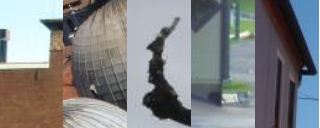
\includegraphics[width=0.8\textwidth]{lbp_fps.png}
\caption{Przykłady fałszywie pozytywnych detekcji w metodzie LBP}
\label{fig:fp_lbp}
\end{figure}

\begin{center}
    \begin{longtable}{ | p{5cm} | p{3cm} | p{3cm} |}
     \caption{Ilość znalezionych fałszywie pozytywnych okien przy użyciu deskryptora zbudowanego na podstawie macierzy kowariancji} \\
    \hline
	Rozmiar bloku & 32x32 & 64x64\\ \hline
	Funkcja jądra SVM & liniowa & liniowa   \\ \hline
    Ilość znalezionych pozytywnie fałszywych okien & 4711 & 5292 \\ \hline
    \end{longtable}
    \label{tab:fp_lbp}
\end{center}

\subsection{Wyniki drugiej walidacji}

W tabeli \ref{tab:lbp_second} zestawiono wyniki krzyżowej walidacji klasyfikatora po dotrenowaniu pierwszego klasyfikatora fałszywymi pozytywnymi detekcjami, wykrytymi w zbiorze testowym. W celu zminimalizowania efektu przetrenowania klasyfikatora wzięto pod uwagę 25\% fałszywie pozytywnych detekcji wygenerowanych na zbiorze testowym.

\begin{center}
    \begin{longtable}{ | p{5cm} | p{3cm} | p{3cm} |}
    \caption{Wyniki drugiej walidacji krzyżowej przy użyciu deskryptora LBP}
    \label{tab:lbp_second}\\
    \hline
	Rozmiar bloku & 32x32 & 64x64 \\ \hline
	Funkcja jądra SVM & liniowa & liniowa  \\ \hline
    Liczba pozytywnych detekcji w pozytywnym zbiorze testowym & 479 & 512 \\ \hline
    Liczba negatywnych detekcji w pozytywnym zbiorze testowym & 147 & 134 \\ \hline
    Celność metody w pozytywnym zbiorze testowym & \textbf{76,52\%} & \textbf{81,79\%} \\ \hline
    Liczba pozytywnych detekcji w negatywnych zbiorze testowym & 3 & 30 \\ \hline
    Liczba negatywnych detekcji w negatywnym zbiorze testowym & 903 & 876 \\ \hline
    Celność metody w negatywnym zbiorze testowym & \textbf{99,67\%} & \textbf{96,69\%} \\ \hline
    \end{longtable}
\end{center}


\subsection{Rozkłady błędów detekcji}

Wykres rozkładu błędu detekcji zaprezentowany został na rysunku \ref{fig:lbp_det}. Analizując wykres można dojść do wniosku, że oba przetestowane wielkości bloków, w których liczonych jest histogram metody LBP dają zbliżone do siebie rezultaty pod kątem celności detekcji.

\begin{figure}[htb]
\centering
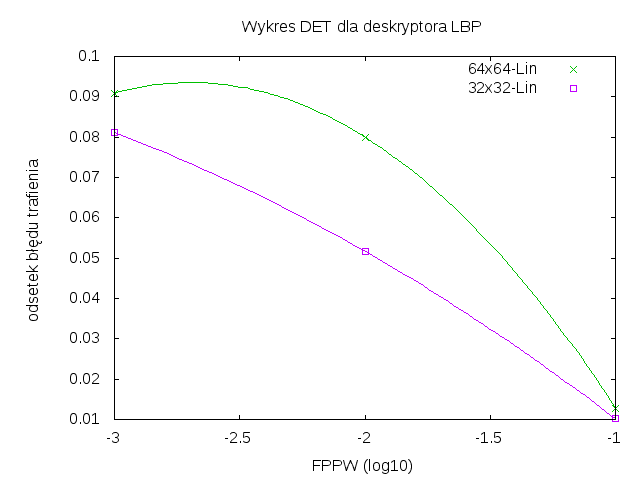
\includegraphics[width=0.9\textwidth]{lbp_det.png}
\caption{Rozkład błędu detekcji dla różnych przyjętych wielkości bloków}
\label{fig:lbp_det}
\end{figure}

\subsection{Analiza złożoności poszczególnych kroków metody}

W tabeli \ref{tab:lbp_times} zestawiono czasy wykonywania poszczególnych kroków metodologii, w zależności od rozmiaru bloku, w której wyliczany jest histogram metody LBP.

\begin{center}
    \begin{longtable}{ | p{5cm} | p{3cm} | p{3cm}|}
     \caption{Czas wykonywania poszczególnych etapów badania metody LBP} 
     \label{tab:lbp_times}\\
    \hline
	Rozmiar bloku & 32x32 & 64x64 \\ \hline
	Funkcja jądra SVM & liniowa & liniowa  \\ \hline
    Ekstrakcja cech pozytywnych / próbka & 14,10 ms & 11,08 ms \\ \hline
    Ekstrakcja cech negatywnych / próbka & 12,42 ms & 10,19 ms \\ \hline
    Pierwszy trening klasyfikatora & 79 s & 27,67 s \\ \hline
    Generacja fałszywie pozytywnych okien & 917,78 s & 657 s \\ \hline
    Drugi trening klasyfikatora & 89,83 s & 31,62 s \\ \hline
    Analiza rozkładu błędu detekcji w zbiorze testowym & 4831 s & 4914 s \\ \hline
    \end{longtable}
\end{center}


\subsection{Podsumowanie}
Podsumowując przeprowadzone testy, można zauważyć że pod względem jakościowym oba przetestowane rozmiary bloku, w którym na obrazie wyliczany jest histogram rozkładu wzorca, dają podobne rezultaty. W przypadku bloku 32x32 piksele jednak, poziom detekcji jest nieco wyższy w przypadku gdy rząd FPPW wynosi $10^{-2}$. Biorąc jednak pod uwagę rozmiar wektora cech, jaki powstaje przy ich ekstrakcji, słuszniejszym wyborem wydaje się być blok o rozmiarze 64x64, gdzie długość wektora cech jest 4 mniejsza od bloku 32x32. W konsekwencji, trening SVM zajmuje krótszy czas.

\clearpage

\section{Edgelets}
\label{sec:edge}

\subsection{Wprowadzenie}
Algorytm zaproponowany przez autorów metody, B. Wu i R. Nevatię w pracy \cite{Wu05} nie jest typowym deskryptorem cech opisującym obraz w postaci wektora. Zaproponowana metoda polega na budowie kaskadowego klasyfikatora, porównującego w każdym kroku podobieństwo fragmentu obrazu do każdego z wielu przygotowanych wcześniej wzorcowych kształtów. Ponieważ SVM, klasyfikator używany w tej pracy, jest mocnym klasyfikatorem, potrzebującym do treningu i klasyfikacji wektora zawierającego całość informacji, w niniejszej pracy dokonana została próba przystosowania metody do użycia właśnie z wykorzystaniem takiego rodzaju klasyfikatora.

Ze względu na bardzo wysoką złożoność metody, w przypadku porównywania z wieloma wzorcowymi kształtami, na podstawie zbioru treningowego, wygenerowano po 150 losowych masek dla fragmentów obrazu o rozmiarze 3x3, 4x4 i 5x5 i na ich podstawie dokonywano obliczenia deskryptora.


\subsection{Algorytm obliczenia deskryptora}

Proponowany algorytm obliczenia deskryptora cech, bazujący na oryginalnej metodzie \textit{Edgelets} ma następującą postać:

\begin{algorithm}[H]
 \SetAlgoLined
 \KwData{obraz $n x m$ w przestrzeni barw RGB;\\$k$ - rozmiar maski, względem której dokonywane jest porównywanie;\\macierz wzorcowych masek ($l x k^2$)}
 \KwResult{wektor deskryptora cech o długości $l$}
 zamień przestrzeń barw RGB na skalę szarości\;
 oblicz gradient w obu kierunkach na obrazie np. używając maski  $\left[\begin{array}{ccc}1 & 0 & -1\end{array}\right]$\;
 oblicz długość wektora gradientu w każdym pikselu\;
 dokonaj dyskretyzacji kąta gradientu w każdym pikselu: $round(\frac{atan2(I_y, I_x)*6}{\pi})$\;
 $L := [1, 0.8, 0.5, 0, 0.5, 0.8]$\;
 \ForEach{pikselobrazu $\in$ obraz, pikselobrazu $\in \{0,1,..,5\}$}{
	\ForEach{maska wzorcowa} {
	ocena := 0\;
		\ForEach{pikselmaski $\in$ maska, pikselmaski $\in \{0,1,..,5\}$}{
			ocena := ocena + $\sqrt{I_x^2+I_y^2} * L[\vert piksel obrazu - piksel maski\vert+1]$\; 
		}
	wektor(maska) := wektora(maska) + ocena\;
	}
 }
 \Return{wektor cech}\;
 \caption{Proponowany algorytm deskryptora cech, wykorzystujący metodę Edgelets}
\end{algorithm}

\subsection{Wyniki pierwszej walidacji}

W tabeli \ref{tab:edge_first} zestawiono wyniki krzyżowej walidacji klasyfikatora wytrenowanego 
próbkami, uzyskanymi na podstawie wyliczenia wyżej zaproponowanego deskryptora cech, w zależności od rozmiaru fragmentów obrazu, które były porównywane.

\begin{center}
    \begin{longtable}{ | p{5cm} | p{3cm} | p{3cm} | p{3cm} |}
    \caption{Wyniki walidacji krzyżowej przy użyciu proponowanego deskryptora bazującego na metodzie \textit{Edgelets}}
    \label{tab:edge_first}\\
    \hline
	Rozmiar fragmentu & 3x3 & 4x4 & 5x5 \\ \hline
	Funkcja jądra SVM & liniowa & liniowa & liniowa  \\ \hline
    Długość wektora cech & 150 & 150 & 150 \\ \hline
    Liczba pozytywnych detekcji w pozytywnym zbiorze testowym & 615 & 97 & 468 \\ \hline
    Liczba negatywnych detekcji w pozytywnym zbiorze testowym & 11 & 529 & 158 \\ \hline
    Celność metody w pozytywnym zbiorze testowym & \textbf{98,24\%} & \textbf{15,50\%} & \textbf{74,76\%} \\ \hline
    Liczba pozytywnych detekcji w negatywnych zbiorze testowym & 650 & 362 & 476 \\ \hline
    Liczba negatywnych detekcji w negatywnym zbiorze testowym & 256 & 544 & 430 \\ \hline
    Celność metody w negatywnym zbiorze testowym & \textbf{28,26\%} & \textbf{60,04\%} & \textbf{47,46\%} \\ \hline
    \end{longtable}
\end{center}

\subsection{Analiza złożoności poszczególnych kroków metody}

\begin{center}
    \begin{longtable}{ | p{5cm} | p{3cm} | p{3cm} | p{3cm} |}
    \caption{Czas wykonywania poszczególnych etapów badania metody opartej na metodzie \textit{Edgelets}}
    \label{ref:edge_times}\\
    \hline
	Rozmiar fragmentu & 3x3 & 4x4 & 5x5 \\ \hline
	Funkcja jądra SVM & liniowa & liniowa & liniowa  \\ \hline
    Ekstrakcja cech pozytywnych / próbka & 118,31 ms & 158,6 ms & 114,40 ms \\ \hline
    Ekstrakcja cech negatywnych / próbka & 100,46 ms & 161,40 ms & 136,56 ms \\ \hline
    Pierwszy trening klasyfikatora & 0,67 s & 1,29 s & 0,98 s \\ \hline
    \end{longtable}
\end{center}


\subsection{Podsumowanie}
Uzyskanie nieobiecujących wyników w walidacji krzyżowej dla danej metody, a także jej bardzo duża złożoność poskutkowały zaniechaniem dalszych badań. Dodatkowo, informacje na podstawie jakich budowany jest wektor deskryptora (gradient obliczony na obrazie) brane są pod uwagę w innych, mniej złożonych i skuteczniejszych metodach takich jak HOG czy uzyskującej wektor cech z macierzy kowariancji. Takie podejście opisu obiektu zatem nie sprawdza się w przypadku, gdy do klasyfikacji używamy mocnych klasyfikatorów, takich jak Support Vector Machine.

\section{Zestawienie przebadanych metod}

Wspólny wykres, dla najlepszych wariantów każdej z metod przedstawiono na rysunku \ref{fig:joint_det}. Można z niego wywnioskować, że wszystkie z przebadanych metod, dla przyjętej w tej pracy metodologii, reprezentują podobny poziom detekcji dla FPPW tego samego rzędu. Najlepszą z przebadanych metod, w kontekście detekcji ludzi, bazując na wynikach rozkładu, jest metoda HOG. Należy jednak pamiętać, że została ona zaprojektowana \textit{stricte} dla detekcji sylwetek ludzkich na obrazie, podczas gdy dwie pozostałe są metodami bardziej uniwersalnymi.

\begin{figure}[htb]
\centering
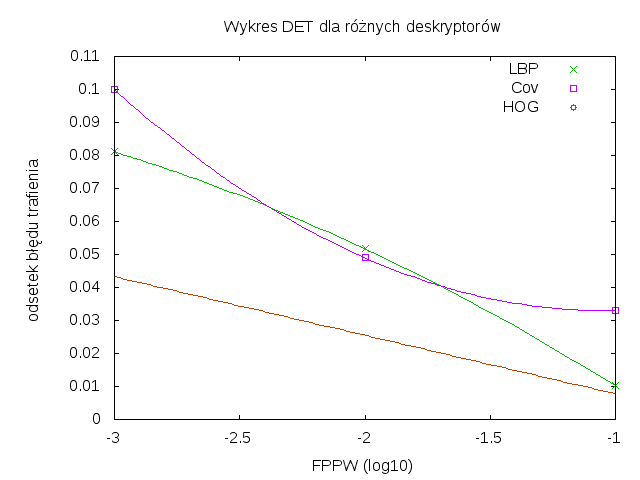
\includegraphics[width=0.8\textwidth]{joint_det.png}
\caption{Wspólny wykres DET dla przebadanych metod}
\label{fig:joint_det}
\end{figure}